\documentclass{article}

\usepackage[final]{neurips_2019}

\usepackage[utf8]{inputenc}
\usepackage[T1]{fontenc}
\usepackage{hyperref}
\usepackage{url}
\usepackage{booktabs}
\usepackage{amsfonts}
\usepackage{nicefrac}
\usepackage{microtype}
\usepackage{graphicx}
\usepackage{xcolor}
\usepackage{lipsum}
\usepackage{multirow}

\newcommand{\note}[1]{\textcolor{blue}{{#1}}}

\title{
  Whiskey GPTaster \\
  \vspace{1em}
  \small{\normalfont Stanford CS224N Custom Project}  % Select one and delete the other
}

\author{
  Akram Sbaih \\
  Department of Computer Science \\
  Stanford University \\
  \texttt{akram@stanford.edu} \\
  % Examples of more authors
   \And
   \texttt{Mentor} John Hewitt \\
   Department of Computer Science \\
   Stanford University \\
   \texttt{johnhew@stanford.edu} \\
%   \And
%   Name \\
%   Department of Computer Science \\
%   Stanford University \\
%   \texttt{name@stanford.edu}
}

\begin{document}

\maketitle

\begin{abstract}
Recent works in language modeling and text generation started raising concerns on the potential for machines to generate fake news and reviews. These models now generate text shown to be indistinguishable from human text \cite{adelani2019generating}. Some recent approachs \cite{zellers2020defending} train classifiers to discriminate fake and real text. These usually require access to the generator or its training data which aren't usually available in the wild. We're also faced with the constraint of having few examples of identifiable good fakes. In this work, I study the performance of classifiers with combinations of [the generator, its training data, its generations]. To this end, I generated a set of fake whiskey reviews using GPT2 to evaluate these approachs. I found that access to the trained parameters of the generator didn't improve classification.
\end{abstract}

\note{Code available at \href{https://github.com/aksbaih/reviews-generation}{https://github.com/aksbaih/reviews-generation}}

\section{Introduction}
The spread of the COVID-19 Pandemic has lead to increase in online shopping \cite{covidincrease}. With the lack of other references, people rely on online reviews to decide before purchising online items. For example. customers are 270\% more likely to buy a product with reviews than another without \cite{reviews270}. This means that reviews have a great financial power online. In this project, we will be exploring methods to automatically generate such reviews and then to detect their legitmacy. We are especially interested in the potential use of publicly available technologies to do this, and how much we need to know about he generator to detect its generations. This is because we usually don't have access to the generator or many of its generations in the real world when we try to decide on the legitmacy of a review.

\section{Related Works}
The recent advancements in transformers and language modeling introduced big and powerful models that are available for the public such as \cite{gpt}\cite{t5}\cite{bert}. These models can be trained to generate fake text possibly conditioned on some tasks. We will make use of GPT-2, a language model, to generate a dataset of fake reviews which we will use to train a classifier on fake/real detection. \\\\
This lead to the need for an automated method to detect machine-generated text and distinguish it from human-generated text. This is especially a hard task given how similar these machine generations are to human text \cite{adelani2019generating} that even humans can't distinguish them. Some approaches \cite{zellers2020defending} use the trained generator as a tool to identify its own generations. However, these trained generators are not publicly available and therefore we need to assess approaches that use minimal information about the generator. In this project, I will be exploring and evaluating three approaches which I introduce in the following section.


\section{Approach}
The goal is to make a classifier that takes in a Whiskey review and decides whether it's human generated or machine generated.  In this project, I define a human-generated review as one that has been scraped from a crowdsourced dataset, while a machine-generated review is one made by GPT2 finetuned on that human dataset. These definitions reflect only a small combination of the potential samples in the wild, but still serve as a good evaluation since GPT2 is one of the widely-used architectures in the market. To this end, there are multiple approaches that I would like to compare. 
\begin{itemize}
\item Finetune GPT2 to be a classifier that takes these input as a sequence and outputs a token deciding whether the review is real or fake, starting from a publicly available GPT2 checkpoint. This serves as the baseline model.
\item Finetune GPT2 as the previous approach but start from the checkpoint that was used for generation similar to the approach proposed in \cite{zellers2020defending}.
\item Compare the preplexities on the real and generated sequences for both the public and generator-finetuned checkpoints of GPT2 and train a classifier on those preplexities if necessary. 
\end{itemize}
We should expect that all three approaches perform well. However, each of them offers a different set of constraints. For example, we probably will not have access to the finetuned generator in the wild. We also might be faced with a very limited number of fake reviews from the same generator that we can train a classifier on. Therefore, comparing the results of these approaches offers a valuable understanding of what we can and cannot do to combat bad use of language models for generating fake reviews.
\\ To evaluate these approaches, I set the following milestones
\begin{enumerate}
\item Prepare a dataset of human-generated reviews with their metadata.
\item Finetune Huggingface GPT2 on that dataset to generate novel fake reviews making a new fake-reviews dataset.
\item Implement each of the approaches and assess their accuracy.
\end{enumerate}

\section{Generation Experiments}
\paragraph{Data}$ $
\\ \href{www.whiskyadvocate.com}{www.whiskyadvocate.com} is a website where people write their reviews and ratings for various whiskeys. I made a script that scraped all the reviews on the website totaling 5649 unique ones. Each review contains the name of the whiskey, its price in dollars, its rating out of 100, and the text review of its taste.  Some examples are shown in Table \ref{reviewstable}. 
\\ I split the data into train, validation, and test sets being 90\%, 6\%, and 4\% which are 5084, 339, and 226 samples, respectively. I intended for the training split to be bigger than the convention because of the limited number of total samples. The test split is also small because main evaluation done on it will be qualitative which is labor-intensive. 
\\ The reviews are reformatted as sequences to be fed into GPT2. An example of the formatting I used is \texttt{"<price>105<rating>89<whiskey>Springbank 11 year old, 58\%<review>Finished in a rum cask. Gently sweet [...] exclusive.)"} where \texttt{[...]} indicates omitted text.

\paragraph{Evaluation method}$ $
\begin{enumerate}
\item Preplexity. This is the average uncertainity the language model has over the sequence it's evaluated on (the lower the better). Since GPT2 is a language model, I used this metric to track how well it's adapting to the new task of modeling whiskey reviews during finetuning. It's also a measure of how well the the final model performs.
\item Qualitative assessment. Since I don't have access to enough labor-work to turn human assessment of the generations into a quantative measure like in \cite{adelani2019generating}, I resorted to my personal assessment. This involves looking at the generated samples for common themes in whiskey reviews. This includes things like having a description of common flavors, distinction between nose and palate, having an after-tast, and mentioning the name of the whiskey in the review. 
\item Accuracy. This is useful for the classifiers proposed in the approach section.
\end{enumerate}

\paragraph{Experimental details}$ $
\\ After preprocessing the dataset, I ran the Huggingface GPT2 Trainer on the training and validation splits for 5 epochs starting with their publicly available pre-trained GPT2 checkpoint. I chose a batch size of 2 per device beecause of the limited available memory. Each sample in the batch is the sequence concatenation of multiple samples from the training set so that we use up all the available GPT2 block size and train faster. 
\\ I trained on an Azure machine with two K-80's making a total batch size of 4 with 4 dataloading workers. I used the default learning rate of $5e-5$ and the default Cross Entropy loss function. Training took 31 minutes and ended up with a preplexity of 15.49 on the validation set.  You can see the loss curve in Figure \ref{Fig:get_finetune_loss_fig}.

\begin{figure}[tb]
 \centering
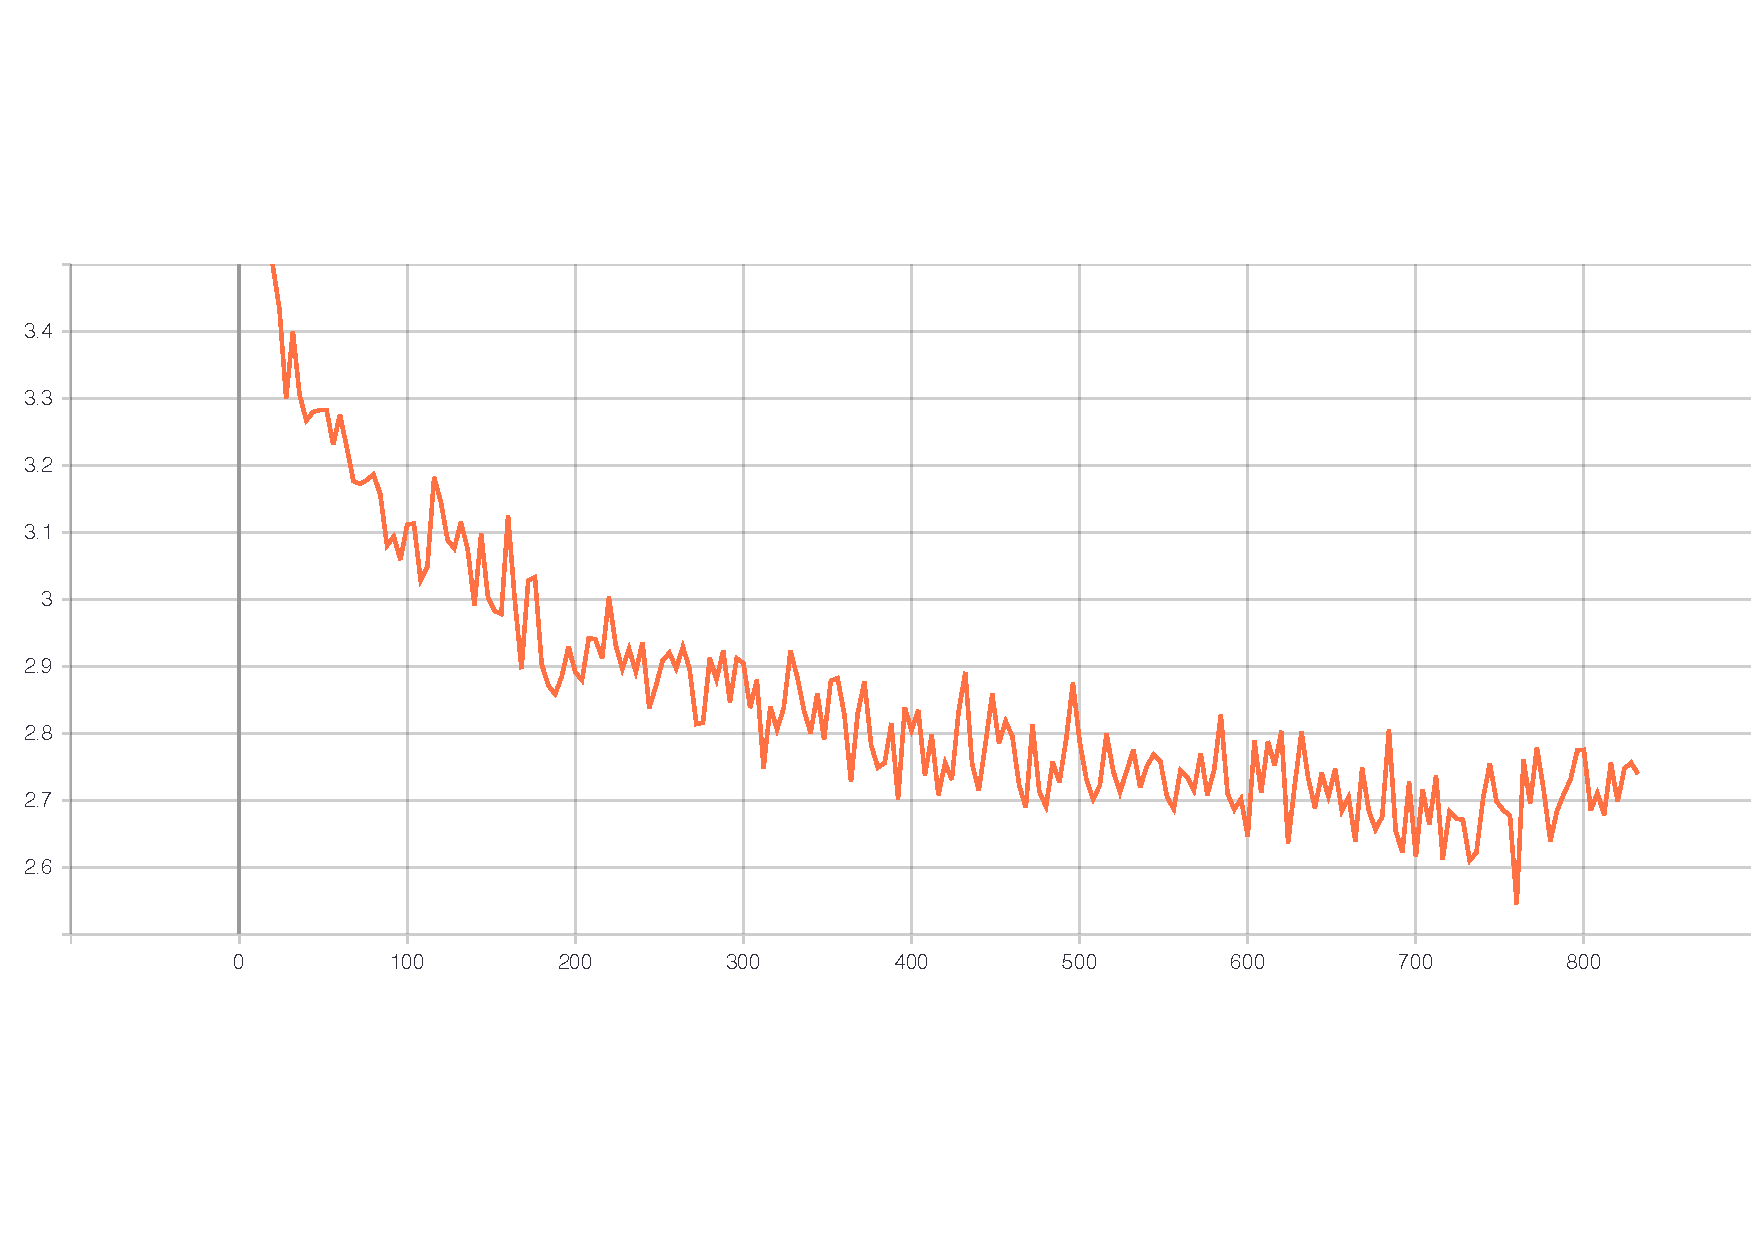
\includegraphics[width=0.7\columnwidth]{finetune_condgen_train_loss.pdf}
\vspace{-12mm}
\caption{GPT2 Training Loss for 5 epochs.}
\label{Fig:get_finetune_loss_fig}
\vspace{-3mm}
\end{figure}

\paragraph{Results}$ $
\\The baseline for the generation task is the human generated text since we're not comparing the model to other models because that's not the goal of this project. I use my human evaluation to look for common patterns in the generated text as mentioned in the Evaluation Method section.  The generations seem satisfying except for an observation that the model tends to list too many flavors sometimes. Table \ref{reviewstable} shows a few randomly selected generations from the test set.

\section{Classification Experiments}$ $
\\In the previous section, I discussed how to generate fake reviews. In this section, I will be experimenting with the proposed approaches to classify these revies into fake and real.

\paragraph{Data}$ $
\\ The generator has not been trained on the validation and test splits of the original scraped dataset. Therefore, I use these two splits to construct the classification dataset consisting of 565 reviews.  Alongside the real reviews, I add the fake reviews generated by the generator on the validation and test set, adding another 565 fake reviews. We can always generate more fake reviews to make the dataset bigger, but these numbers keep a balance between the reals and the fakes. Finally, the total dataset of 1130 fake/real reviews is split into train/val/test sets of ratios 90\%/6\%/4\% or 1017/68/45 reviews respectively.

\paragraph{Evaluation method}
\begin{itemize}
\item Percision. This is a measure of how much of the predicted fakes are actually fake. We want to find fake reviews but we also don't want real reviews misclassified as fake.
\item Recall. This is a measure of how much of the actually fake reviews the classifier flags as fake. We don't want a classifier that misses a lot of fakes.
\item Accuracy. This is a more common measure worth measuring as it shows how much of the predictions are correct.
\end{itemize}

\paragraph{Experimental details}$ $
\\We're experimenting with three approaches with the following details for each one.
\begin{enumerate}
\item \textbf{Public Checkpoint} baseline. In this approach, I take a publicly available checkpoint on GPT-2 and finetune it to predict fake and real reviews by generating a specific token. I train the model by entering the review as a sequence in the form \texttt{<review>\{ review text \}<pred>\{ fake/real \}<|endoftext|>}. I trained it for 50 epochs on the same hardware as the generator taking 90 minutes.  Training is shown in \ref{Fig:classifier_loss} and results in \ref{Tab:classifier_metrics}.
\item \textbf{Private Checkpoint}. This approach is the same as the previous one except for the fact that it starts training from the last checkpoint of the generator model. The motivation for this approach is that training the generator added useful prior to the model that it could reuse to identify fake review generated by that generator. Training is shown in \ref{Fig:classifier_loss} and results in \ref{Tab:classifier_metrics}.
\item \textbf{Preplexity Approach}.  No training is involved in this one. Instead, both the public and private checkpoints (with no further training) are used to find the perplexity on the review text. The motivation is that the model would be more confident about sequences that it generated than on human-generated text. Results are shown in \ref{Fig:perplexity}.
\end{enumerate}


\begin{figure}[tb]
\vspace{2mm}
 \centering
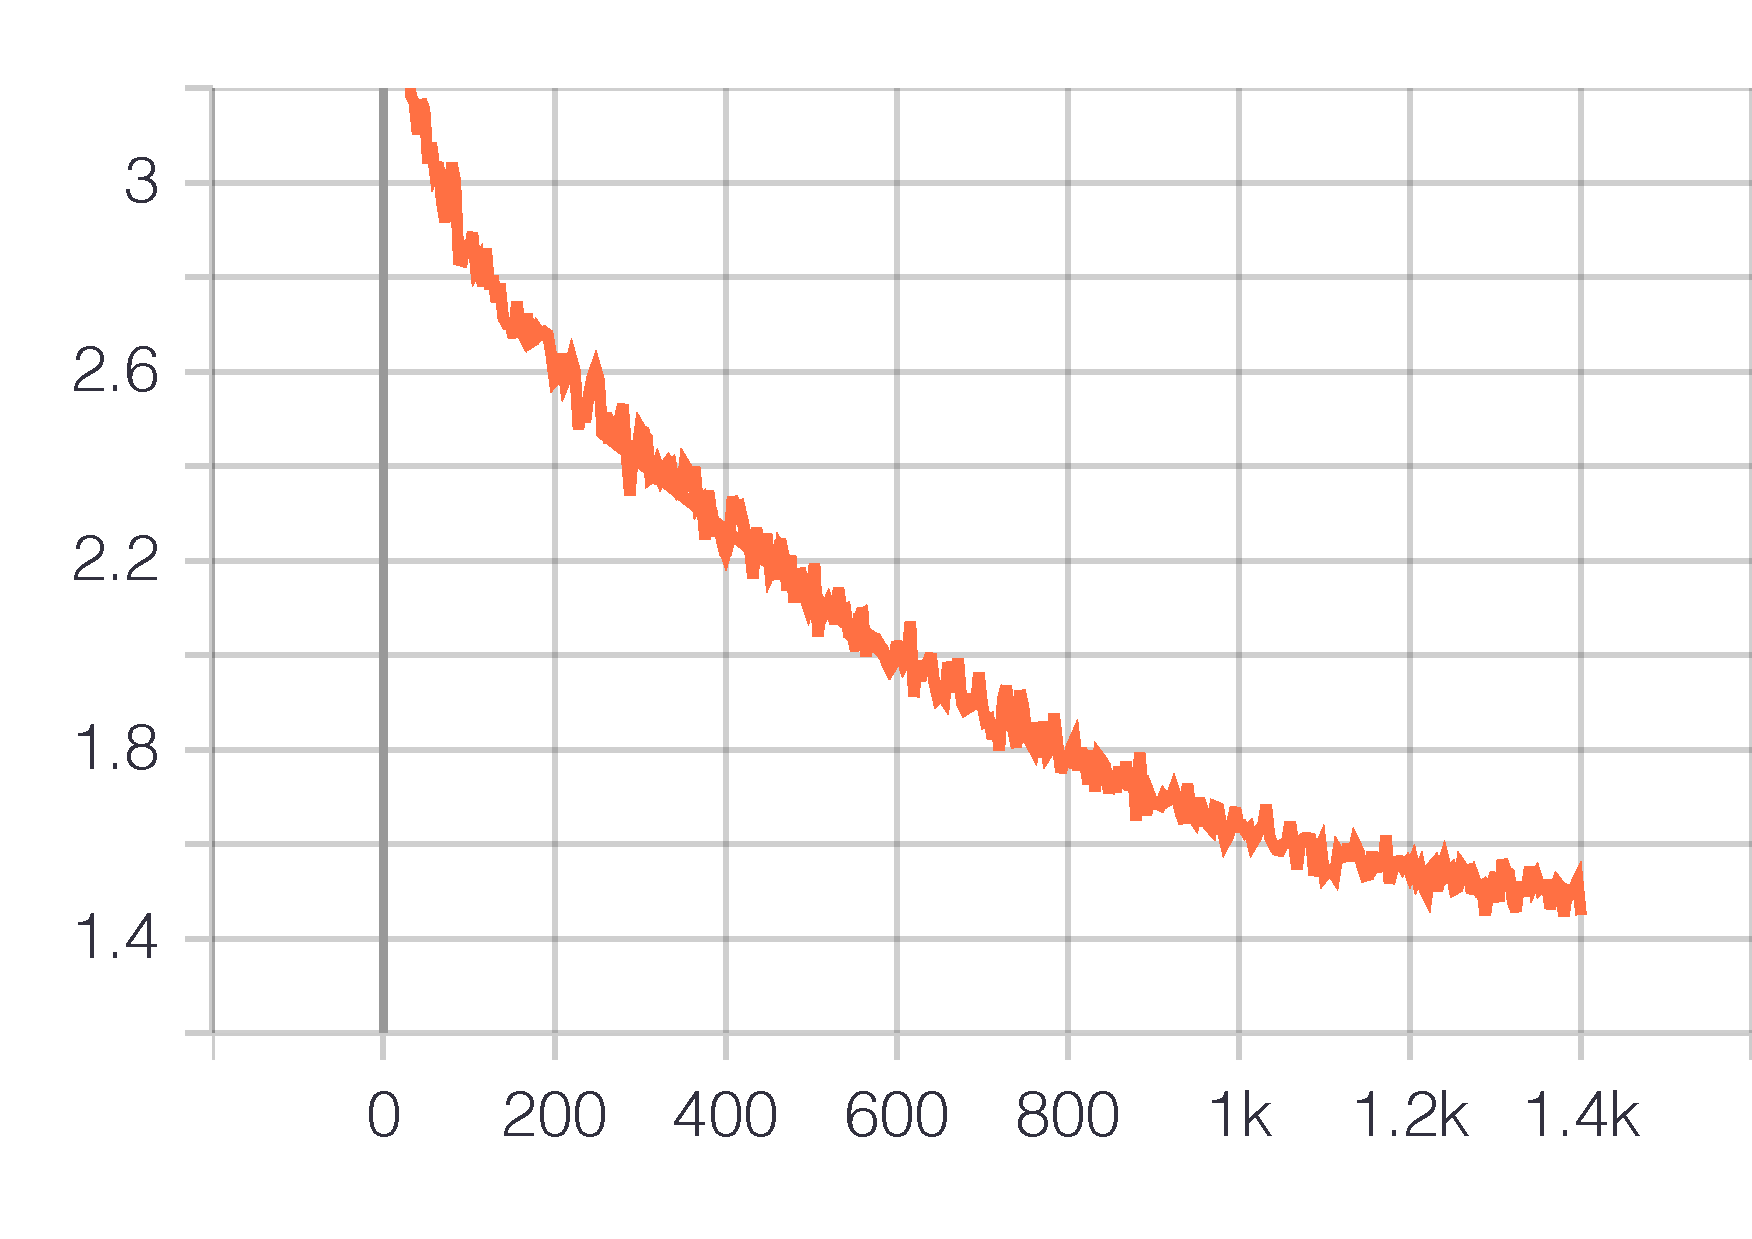
\includegraphics[width=0.24\columnwidth]{train_loss_public}
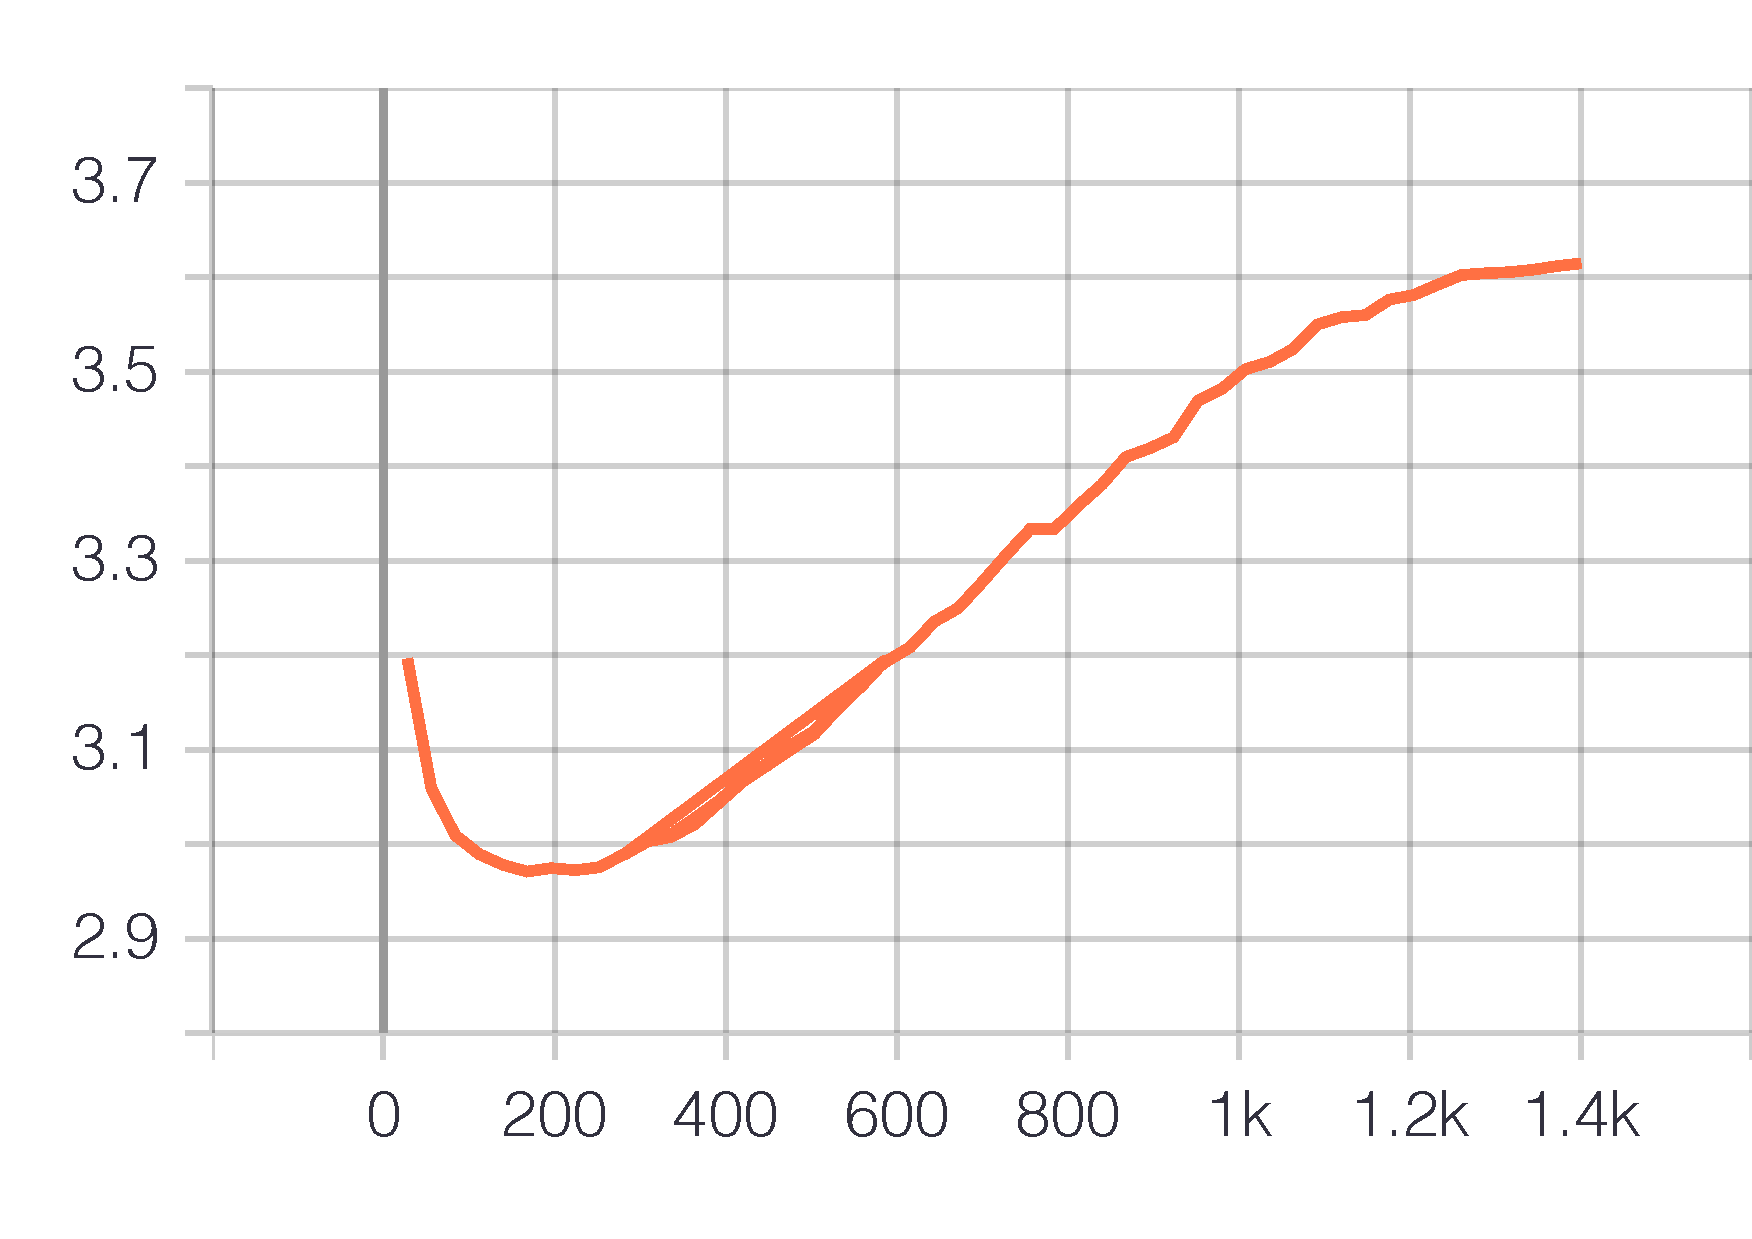
\includegraphics[width=0.24\columnwidth]{eval_loss_public}
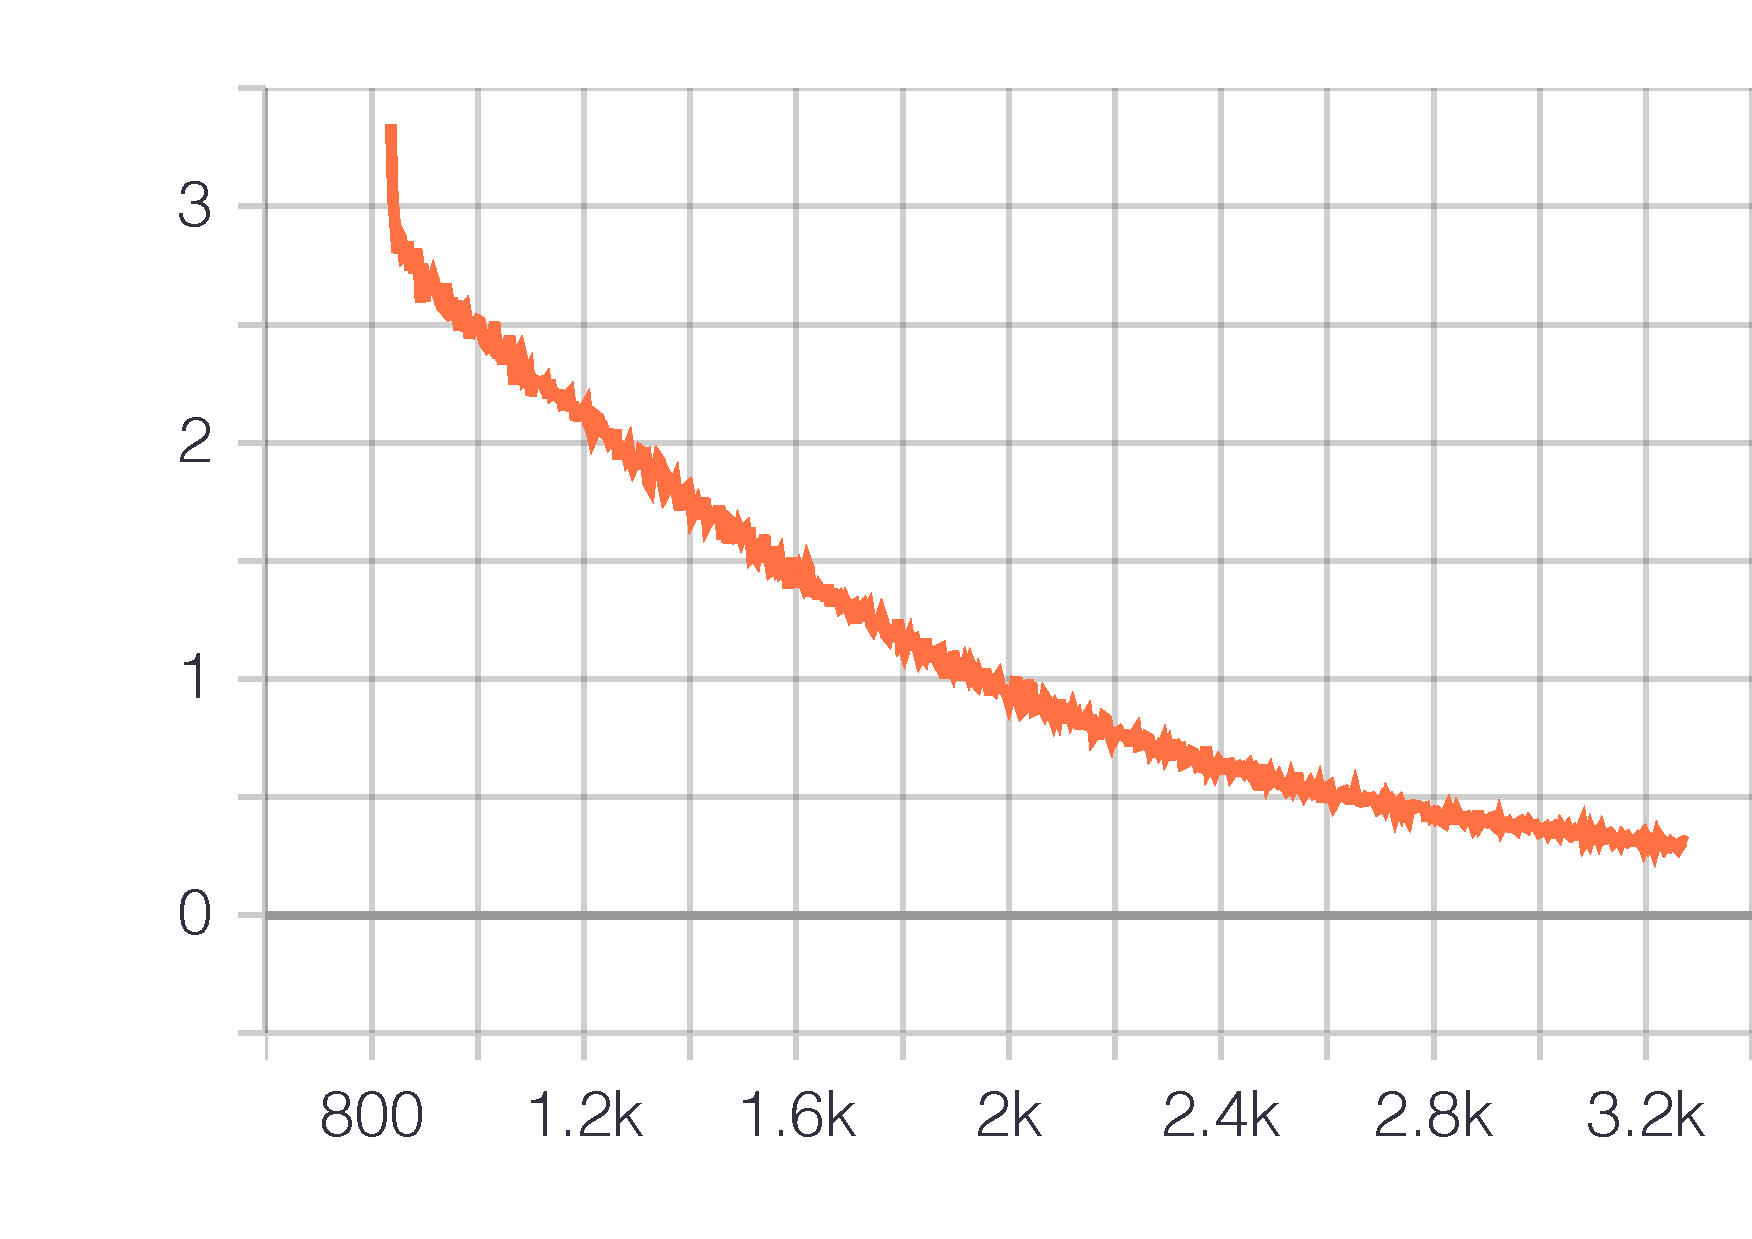
\includegraphics[width=0.24\columnwidth]{train_loss_checkpoint}
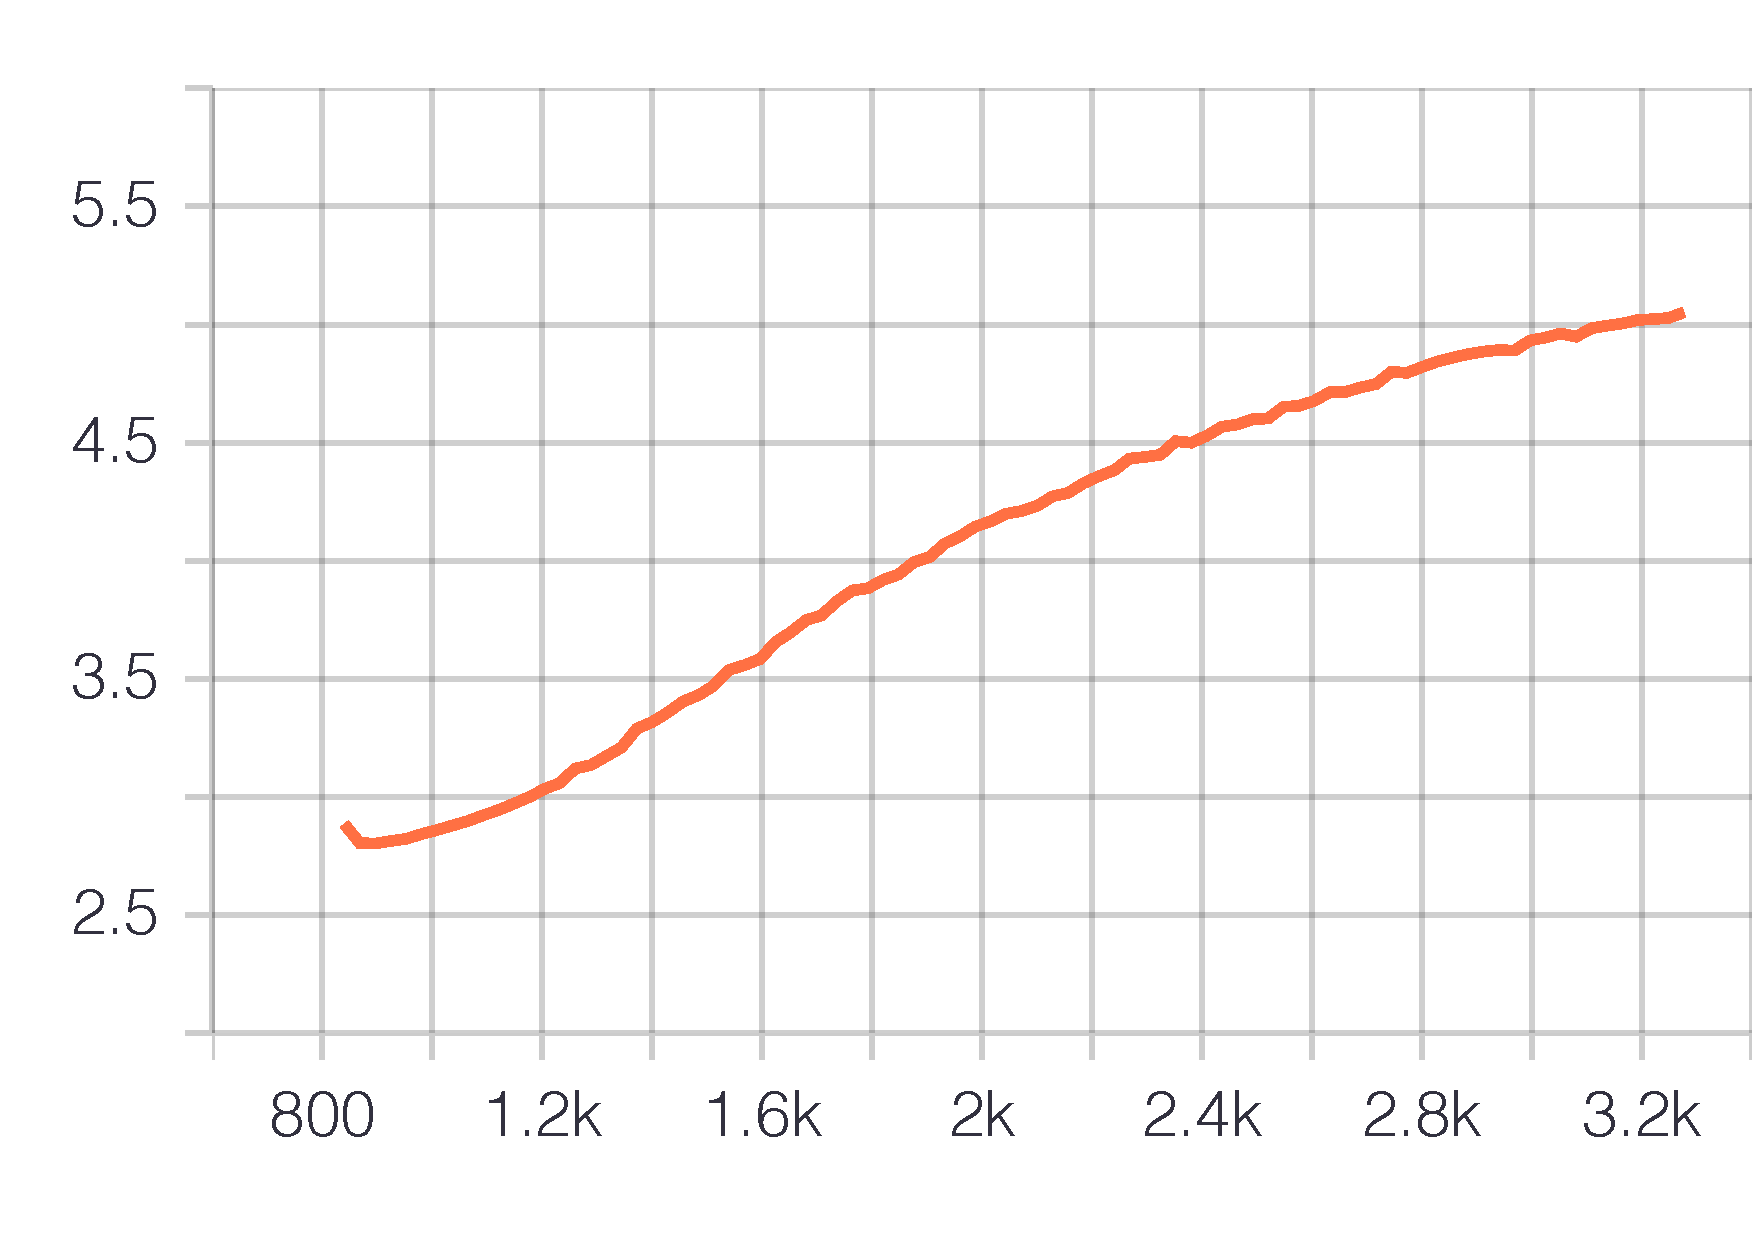
\includegraphics[width=0.24\columnwidth]{eval_loss_checkpoint}
\vspace{-1mm}
\caption{From left to right: public training loss, public validation loss, private training loss, private validation loss. Notice the overfitting happening earlier and worse in the private checkpoint than the public checkpoint.}
\label{Fig:classifier_loss}
\vspace{-3mm}
\end{figure}

\begin{table}[t]
    \vspace{1em}
    \centering
    \scalebox{1}{
   \begin{tabular}{p{32mm} lcclcc}
   \toprule
    \multirow{2}{*}{Model}  & \multicolumn{2}{c}{Public Checkpoint} &  &   \multicolumn{2}{c}{Private Checkpoint}    \\ 
     & Final & Best-Val  & &   Final & Best-Val \\
    \midrule
    Precision          & $62.5$   &  $\textbf{62.9}$ & &  $\textbf{62.9}$   &  
    $61.9$  \\
    Recall          & $80.0$   &  $\textbf{88.0}$  &  & $\textbf{88.0}$   &  
    $52.0$ \\
    Accuracy         & $63.0$   &  $\textbf{65.2}$ &  &  $\textbf{65.2}$   &  $56.5$   \\
    \bottomrule
    \end{tabular}
    }
    \vspace{1em}
        \caption{The maximum value for each metric is bolded. Best-Val is a checkpoint taken at the lowest validation loss for the classifier while Final is the one attained at the end of training. A positivee is defined as "Fake"}
    \label{Tab:classifier_metrics}
\end{table}

\begin{figure}[tb]
\vspace{2mm}
 \centering
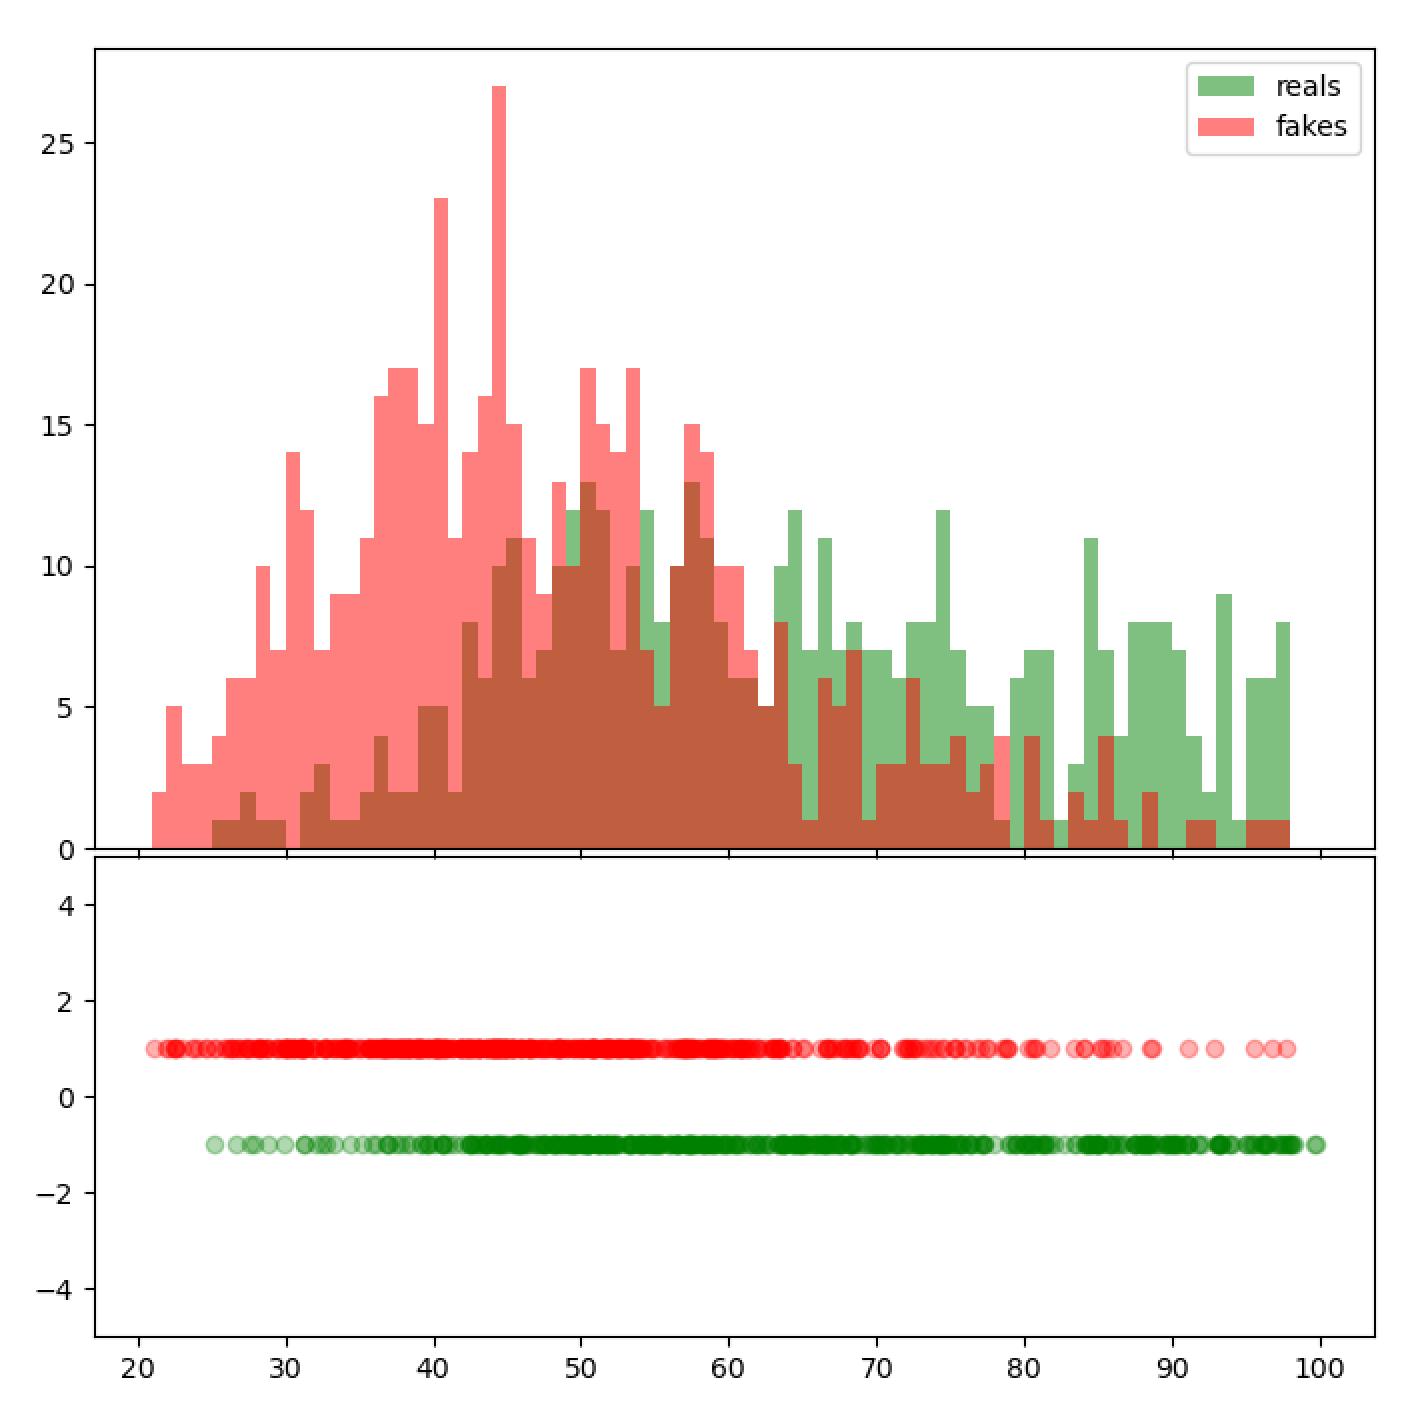
\includegraphics[width=0.45\columnwidth]{public_preplexity}
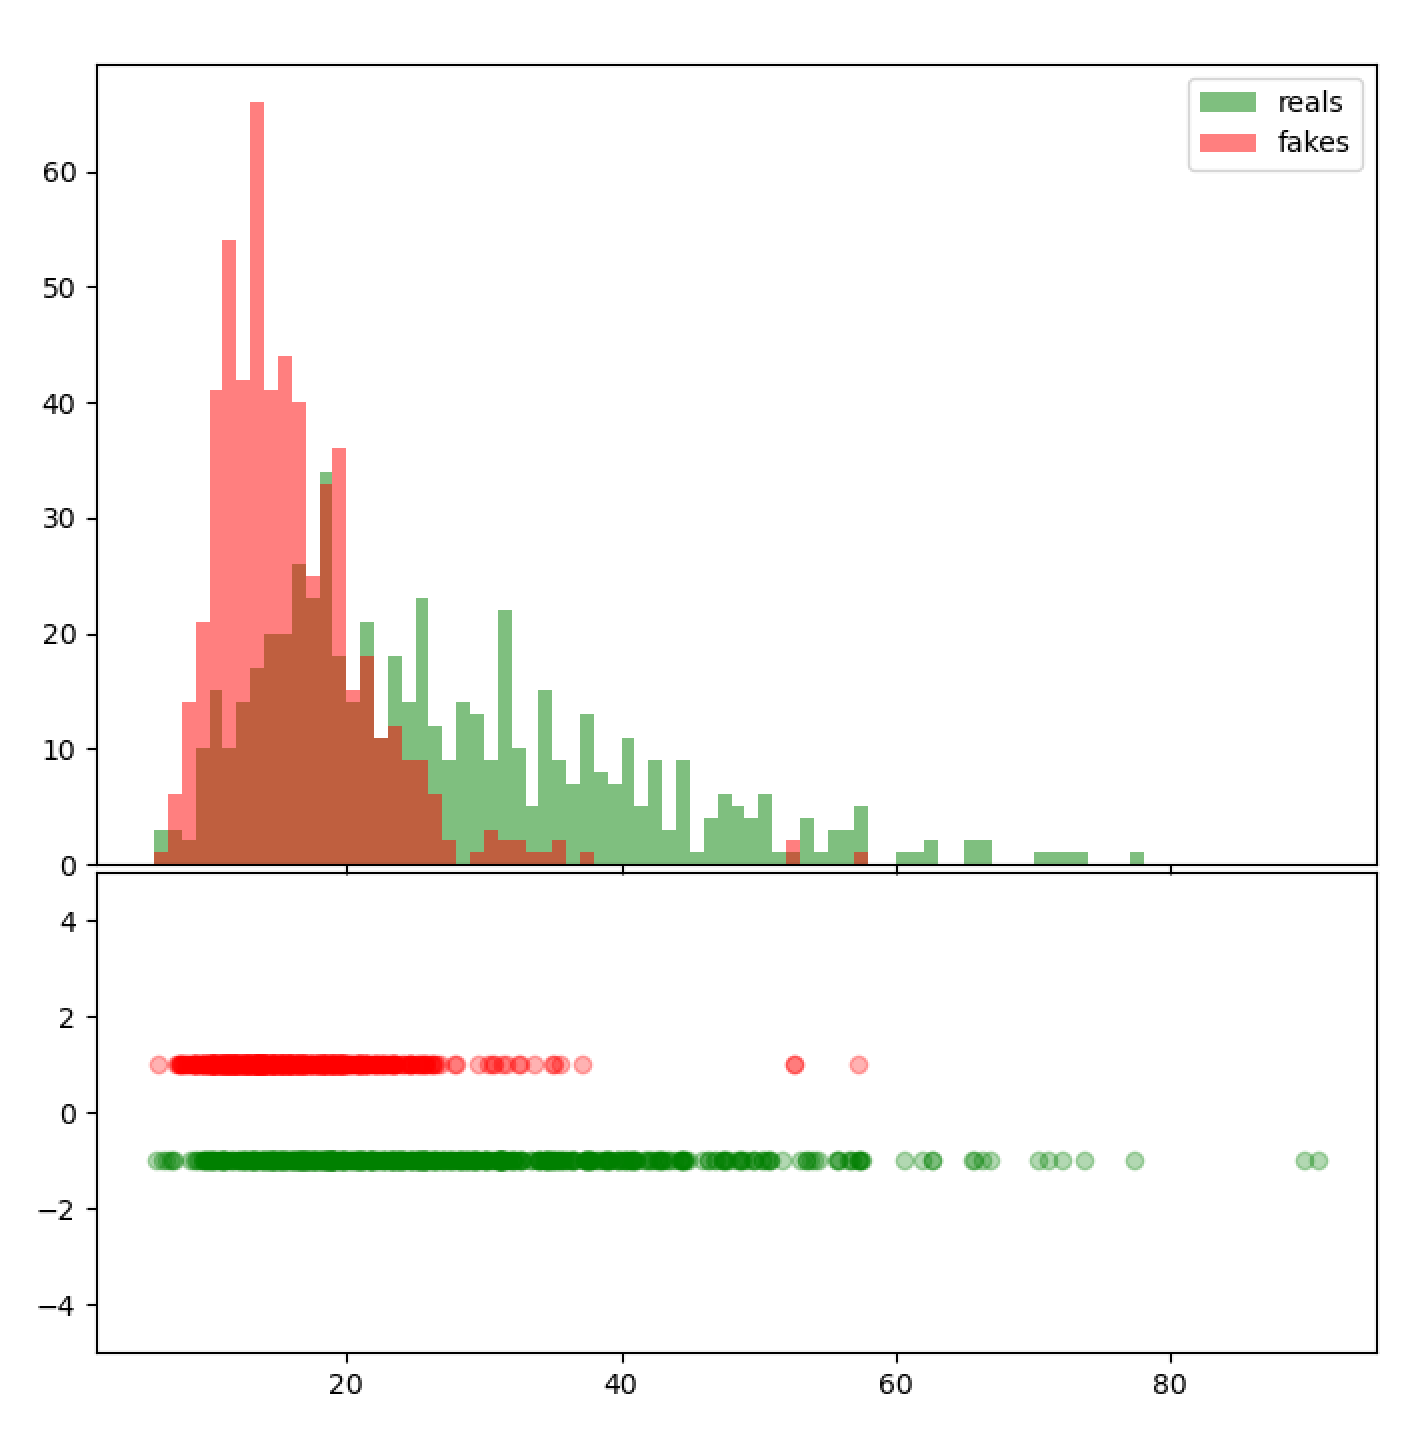
\includegraphics[width=0.45\columnwidth]{private_preplexity}
\vspace{-1mm}
\caption{Public checkpoint on the left and private on the right. Notice the difference is scale.}
\label{Fig:perplexity}
\vspace{-3mm}
\end{figure}

\section{Analysis}$ $
\\ The results are surprising; we see that both the first and second approach reach very similar results at different points. Concretely, we find the following points:
\begin{itemize}
\item Both the Public and the Private approaches start overfitting soon after the first one or two epochs out of 50. This is seen by the increase in validation loss while the training loss is constantly decreasing.
\item The Public checkpoint reaches good results faster than the Private one by the fact that its best validation scores are better than those for the Private approach. This could be due to a need for the Private checkpoint to unlearn the generation task. This result goes against the results of \cite{zellers2020defending}. 
\item The Preplexity approach with its results in \ref{Fig:perplexity} aren't very promising. We notice that the perplexity for fakes is generally lower than the reals, and that the seperation increases for the Private model than the Public one, but there's a lot of overlap between the histograms making it less useful. However, we keep in mind that these results are attained without need for a dataset of fake examples making it useful for scarce scenarios. 
\end{itemize}



\section{Conclusion}$ $
\\The same way we are able to use a language model like GPT2 to generate new fake reviews, we are able to train it with some success to detect these fake texts. Having access to the weights and biases of the generator did not make a difference on how well the model performs. We also explored how other measures like preplexity perform in this task and concluded that they're not as effective, but more work on them could lead to interesting results, especially under constraints like scarcity.




\begin{table}[h]
    \centering
    \begin{tabular}{p{0.48\linewidth} | p{0.48\linewidth}}
        \toprule
        \textbf{Real Example} & \textbf{Fake Example} \\
        \midrule
        <price>495<rating>89<whiskey>Bainbridge Yama American Single Grain Barley Mizunara Japanese Oak Cask, 45\%<review>This high-end whiskey exhibits restrained oak, elegance, and delicateness, with wonderful poached pear, cereal, crème caramel, floral, and lemon chiffon cake aromas that yield to a bright beam of tart, mouthwatering citrus—clementine, lemon, and yuzu—tingling with allspice. Bright, light, and lively, but not lacking in complexity, finishing with marshmallow, toasted almond, and marzipan. Very pretty! American single grain whiskey aged in Japanese Mizunara oak casks.
        &
        <price>495<rating>89<whiskey>Bainbridge Yama American Single Grain Barley Mizunara Japanese Oak Cask, 45\%<review>Distilled in 2003 and bottled in September 2016. Rum mizunara has been a popular whiskey for a very long time, one worth considering. The nose offers light toffee, sweet orange syrup, lime juice, light honey, sandalwood, and light oak, adding some teasing dried spice notes. The palate is spicy, with caramel and milk chocolate, red currant, and dark fruit. It finishes with coffee, orange rind, and cocoa powder, finishing dry and spicy.  \\
        \bottomrule
    \end{tabular}
    \vspace{1em}
    \caption{Real on the left and Fake on the right from the test set.}
    \label{reviewstable}
\end{table}


\bibliographystyle{unsrt}
\bibliography{references}

\end{document}
